\documentclass[UTF8,11pt]{ctexart}
\usepackage[a4paper,margin=2.2cm]{geometry}
\usepackage{amsmath,amssymb}
\usepackage{booktabs}
\usepackage{longtable}
\usepackage{array}
\usepackage{enumitem}
\usepackage{xcolor}
\usepackage{hyperref}
\usepackage{tcolorbox}
\usepackage{tikz}
\usepackage{fontspec}
\usepackage{fancyhdr}
\usepackage{titlesec}
\usepackage{multicol}
\usetikzlibrary{arrows.meta,positioning,shapes.geometric,fit,calc}

\setmainfont{Times New Roman}
\setsansfont{Arial}
\setCJKmainfont{Songti SC}
\setCJKsansfont{PingFang SC}
\hypersetup{
  colorlinks=true,
  linkcolor=blue!50!black,
  urlcolor=blue!55!black,
  citecolor=blue!50!black
}
\pagestyle{fancy}
\fancyhf{}
\lhead{Crypto 入门教学文档}
\rhead{\thepage}
\renewcommand{\headrulewidth}{0.4pt}
\setlist[itemize]{leftmargin=1.6em,itemsep=0.25em,topsep=0.25em}
\setlist[enumerate]{leftmargin=1.8em,itemsep=0.25em,topsep=0.25em}
\titleformat{\section}{\Large\bfseries\sffamily\color{blue!35!black}}{\thesection}{0.6em}{}
\titleformat{\subsection}{\large\bfseries\sffamily\color{blue!45!black}}{\thesubsection}{0.6em}{}
\titleformat{\subsubsection}{\normalsize\bfseries\sffamily\color{black}}{\thesubsubsection}{0.6em}{}

\newtcolorbox{keybox}[1]{
  colback=blue!4!white,
  colframe=blue!45!black,
  title=#1,
  fonttitle=\bfseries\sffamily,
  boxrule=0.6pt,
  arc=1.5mm
}
\newtcolorbox{warnbox}[1]{
  colback=orange!8!white,
  colframe=orange!70!black,
  title=#1,
  fonttitle=\bfseries\sffamily,
  boxrule=0.6pt,
  arc=1.5mm
}
\newtcolorbox{practicebox}[1]{
  colback=green!5!white,
  colframe=green!45!black,
  title=#1,
  fonttitle=\bfseries\sffamily,
  boxrule=0.6pt,
  arc=1.5mm
}

\newcommand{\term}[1]{\textbf{\sffamily #1}}
\newcommand{\timestamp}[1]{\textcolor{blue!50!black}{\texttt{#1}}}

\title{\sffamily\bfseries Cryptocurrency Full Course 2026\\教学笔记与初学者学习路线}
\author{基于 Simplilearn YouTube 视频 \texttt{bRLIeRRV6X4} 的字幕与官方章节整理}
\date{整理日期：2026-06-07}

\begin{document}
\maketitle

\begin{warnbox}{元数据核验}
用户指定的视频是 \href{https://www.youtube.com/watch?v=bRLIeRRV6X4}{Cryptocurrency Full Course 2026 | Cryptocurrency Tutorial For Beginners | Blockchain | Simplilearn}。通过 YouTube MCP 读取到的视频元数据为：
\begin{itemize}
  \item 频道：Simplilearn。
  \item 发布时间：2025-10-20T13:30:30Z。
  \item 时长：约 \(6\) 小时 \(17\) 分 \(43\) 秒。
  \item 标题写作 ``2026''，但描述中写的是 ``Cryptocurrency Full Course 2025''，且实际发布时间不是近三个月。
  \item YouTube MCP 成功读取字幕；由于工具输出层对超长字幕有截断，本文件采用「MCP 字幕证据 + 视频官方章节 + 教学整理」方式写成，不是逐字转录稿。
\end{itemize}
\end{warnbox}

\tableofcontents
\newpage

\section{这门课适合怎么学}

这个视频不是一个纯交易课程，而是一个「crypto 生态总览 + blockchain 开发入门」合集。它覆盖的范围很宽：cryptocurrency、NFT、blockchain、Binance、Fantom、liquidity pool、Ethereum Merge、blockchain developer 路线、Solidity 与智能合约、Pi Network。对小白来说，它最适合拿来建立术语体系，而不是直接照着做投资或交易。

\begin{keybox}{本文件的使用方式}
\begin{enumerate}
  \item 先读第 \ref{sec:map} 节的章节地图，知道视频每段在讲什么。
  \item 再读第 \ref{sec:foundation}--\ref{sec:defi} 节，建立 crypto 基础概念。
  \item 如果你想写代码，再读第 \ref{sec:developer}--\ref{sec:solidity} 节。
  \item 最后读第 \ref{sec:pitfalls} 节，修正视频里过于乐观或已经过时的说法。
\end{enumerate}
\end{keybox}

\section{视频章节地图}
\label{sec:map}

视频官方描述给出的章节如下。注意：这类长视频通常由多个较短教学视频拼接而成，所以不同段落的风格、年份、例子和准确性并不完全一致。

\begin{longtable}{>{\raggedright\arraybackslash}p{2.4cm}>{\raggedright\arraybackslash}p{5.2cm}>{\raggedright\arraybackslash}p{7.1cm}}
\toprule
\textbf{时间戳} & \textbf{官方章节} & \textbf{学习重点} \\
\midrule
\endhead
\timestamp{00:00:00} & Introduction to Cryptocurrency Full Course & Crypto 是什么、课程范围、区块链和数字货币的基本动机。 \\
\timestamp{00:01:50} & What Is NFT And Cryptocurrency & 加密货币、NFT、可替代性与不可替代性的区别。 \\
\timestamp{00:10:37} & What is Blockchain & 区块链作为分布式账本、交易记录、共识与不可篡改性。 \\
\timestamp{00:17:22} & What Is Binance? & 中心化交易所、订单簿、现货/杠杆/期货/P2P 的基本入口。 \\
\timestamp{00:21:59} & What Is Fantom? & Fantom/FTM、DAG、PoS、staking、tokenomics。 \\
\timestamp{00:26:14} & What Is Liquidity Pool? & DeFi 流动性池、AMM、LP、滑点、无常损失。 \\
\timestamp{00:33:19} & What Is Ethereum Merge? & Ethereum 从 PoW 到 PoS 的迁移、能耗和验证者机制。 \\
\timestamp{00:38:51} & How to become Block Chain Developer & 区块链开发者技能路线：密码学、网络、数据结构、Solidity、智能合约。 \\
\timestamp{01:42:37} & Blockchain full course & 更完整的 blockchain/智能合约/工具链课程，包括 Ganache、MetaMask、Remix、Solidity。 \\
\timestamp{06:16:16} & Pi Network Explained & Pi Network、手机挖矿叙事、主网、价格与投机风险。 \\
\bottomrule
\end{longtable}

\section{Crypto 的核心定义}
\label{sec:foundation}

视频开头用一个在线支付失败的故事引出 cryptocurrency。它给出的基本定义是：cryptocurrency 是一种虚拟或数字货币，通常运行在 blockchain 技术之上，用于在线交换、支付或价值转移。

\subsection{更严谨的定义}

对初学者来说，可以把 crypto 拆成三个层次：

\begin{enumerate}
  \item \term{资产层}：Bitcoin、Ether、stablecoin、治理代币、NFT 等。
  \item \term{账本层}：记录谁拥有多少资产、谁向谁转账、交易何时发生。
  \item \term{规则层}：由密码学、共识机制和智能合约决定哪些交易有效。
\end{enumerate}

如果用数学化的记号描述，一个最简账本状态可以写成
\[
S_t = \{(a_i, b_i)\}_{i=1}^n,
\]
其中 \(a_i\) 是账户地址，\(b_i\) 是余额。一次交易 \(Tx\) 会把状态从 \(S_t\) 变成 \(S_{t+1}\)：
\[
S_{t+1} = f(S_t, Tx).
\]
区块链系统的关键问题是：全网如何就 \(S_{t+1}\) 达成一致，并防止有人伪造 \(Tx\) 或重复花同一笔钱。

\begin{figure}[h]
\centering
\begin{tikzpicture}[
  node distance=1.25cm,
  box/.style={draw, rounded corners, minimum width=2.6cm, minimum height=0.8cm, align=center, fill=blue!5},
  arrow/.style={-{Latex[length=2.5mm]}, thick}
]
\node[box] (user) {用户\\钱包};
\node[box, right=of user] (tx) {交易\\签名};
\node[box, right=of tx] (network) {节点网络\\验证};
\node[box, right=of network] (block) {新区块\\写入账本};
\draw[arrow] (user) -- (tx);
\draw[arrow] (tx) -- (network);
\draw[arrow] (network) -- (block);
\end{tikzpicture}
\caption{一笔 crypto 交易的极简流程}
\end{figure}

\subsection{视频中需要纠正的说法}

\begin{warnbox}{不要把宣传语当技术事实}
视频早段提到「cryptocurrency transaction never fails」「手续费几乎没有」「没有限额」。这些说法对小白容易误导。现实中：
\begin{itemize}
  \item 链上交易会因为 gas 不足、nonce 错误、合约 revert、网络拥堵而失败。
  \item Bitcoin、Ethereum 主网在拥堵时手续费可能很高。
  \item 交易所、钱包、国家监管、KYC、AML、提现额度都会形成实际限制。
  \item 加密货币不是天然安全；私钥丢失、钓鱼、恶意合约、交易所破产都是真实风险。
\end{itemize}
\end{warnbox}

\section{Blockchain：分布式账本的结构}

视频在 \timestamp{00:10:37} 之后讲 blockchain。核心思想是：把交易按时间组织成 block，再把 block 串成 chain。每个区块包含上一块的哈希，因此修改旧区块会破坏后续链条。

\subsection{区块的基本结构}

一个简化区块可以写成：
\[
B_k = (\text{prevHash}, \text{timestamp}, \text{transactions}, \text{nonce}, \text{hash}).
\]
其中
\[
\text{hash} = H(\text{prevHash}, \text{timestamp}, \text{transactions}, \text{nonce}).
\]
哈希函数 \(H\) 的性质决定了它适合做链式引用：
\begin{itemize}
  \item 输入稍微变化，输出会显著变化。
  \item 从输出很难反推出输入。
  \item 很难找到两个不同输入产生同一个输出。
\end{itemize}

\begin{figure}[h]
\centering
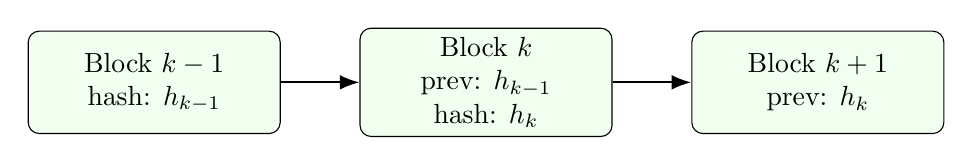
\begin{tikzpicture}[
  block/.style={draw, rounded corners, align=center, fill=green!6, minimum width=3.2cm, minimum height=1.3cm},
  arrow/.style={-{Latex[length=2.5mm]}, thick}
]
\node[block] (b1) {Block \(k-1\)\\hash: \(h_{k-1}\)};
\node[block, right=1.0cm of b1] (b2) {Block \(k\)\\prev: \(h_{k-1}\)\\hash: \(h_k\)};
\node[block, right=1.0cm of b2] (b3) {Block \(k+1\)\\prev: \(h_k\)};
\draw[arrow] (b1) -- (b2);
\draw[arrow] (b2) -- (b3);
\end{tikzpicture}
\caption{区块通过哈希引用前一区块}
\end{figure}

\subsection{去中心化不是没有治理}

视频强调 blockchain 没有中心化第三方。更准确的说法是：它把一部分信任从中心机构转移到协议、密码学、经济激励和节点网络上。不同项目的去中心化程度差异巨大：
\begin{itemize}
  \item Bitcoin 的节点和矿工分布较广。
  \item 某些小链可能由很少验证者控制。
  \item 中心化交易所里的余额不是链上自托管资产，而是交易所数据库里的债权记录。
\end{itemize}

\section{NFT：可替代性与不可替代性}

视频用画家 Susan 的故事解释 NFT。核心概念不是「图片本身不可复制」，而是「链上 token 的所有权记录和元数据可以被验证」。

\subsection{Fungible vs Non-fungible}

\begin{longtable}{>{\raggedright\arraybackslash}p{4cm}>{\raggedright\arraybackslash}p{5.2cm}>{\raggedright\arraybackslash}p{5.2cm}}
\toprule
\textbf{概念} & \textbf{可替代 token} & \textbf{不可替代 token} \\
\midrule
\endhead
英文 & Fungible token & Non-fungible token \\
例子 & \(1\) BTC 与另一个 \(1\) BTC 在账面上等价 & 一个 NFT 与另一个 NFT 通常不等价 \\
价值来源 & 数量、流动性、网络接受度 & 稀缺性、作品、社群、版权/授权、链上记录 \\
交易风险 & 价格波动、交易所风险、流动性风险 & 估值主观、流动性更差、版权误解、项目方风险 \\
\bottomrule
\end{longtable}

\begin{warnbox}{NFT 的常见误解}
NFT 不自动等于版权。买到 NFT 通常只是买到某个链上 token，是否获得图片、音乐、商业使用权，要看项目条款。视频里「NFT 保护艺术品原创性」这个说法需要谨慎理解：NFT 可以证明某个 token 的链上来源，但不能自动阻止别人复制图片文件。
\end{warnbox}

\section{Binance 与中心化交易所}

视频在 \timestamp{00:17:22} 后解释 Binance。它把 Binance 描述为大型 cryptocurrency exchange，提供现货交易、衍生品、staking、P2P 等服务。

\subsection{交易所不是区块链本身}

中心化交易所（CEX）更像一个金融平台。你把钱或币存入交易所，交易所用内部数据库记录你的余额。你在交易所买卖时，很多交易并不会立刻发生在链上，而是在交易所内部订单簿中撮合。

\begin{figure}[h]
\centering
\begin{tikzpicture}[
  node distance=1cm,
  box/.style={draw, rounded corners, align=center, minimum width=3.1cm, minimum height=0.85cm, fill=blue!5},
  danger/.style={draw, rounded corners, align=center, minimum width=3.1cm, minimum height=0.85cm, fill=orange!10},
  arrow/.style={-{Latex[length=2.5mm]}, thick}
]
\node[box] (deposit) {用户充值\\法币或 crypto};
\node[box, right=of deposit] (account) {交易所账户\\内部余额};
\node[box, right=of account] (orderbook) {订单簿\\买单/卖单};
\node[danger, below=of account] (risk) {交易所风险\\冻结、破产、被盗};
\draw[arrow] (deposit) -- (account);
\draw[arrow] (account) -- (orderbook);
\draw[arrow] (account) -- (risk);
\end{tikzpicture}
\caption{中心化交易所的基本结构}
\end{figure}

\subsection{订单簿}

订单簿包含买方愿意出的价格和卖方愿意接受的价格。若最高买价为 \(b\)，最低卖价为 \(a\)，则点差为
\[
\text{spread}=a-b.
\]
点差越大，说明交易成本越高或流动性越差。新手常犯错误是只看币价，不看交易深度、手续费和滑点。

\section{Fantom、DAG 与 Staking}

视频在 \timestamp{00:21:59} 讲 Fantom/FTM，提到 DAG、快速交易、Proof of Stake 与 staking。这里应把它当作「某一类公链项目案例」，不是投资建议。

\subsection{DAG 是什么}

DAG 是 directed acyclic graph，有向无环图。它不是简单的一条链，而是用有方向且无环的图结构记录事件或交易依赖关系。理论上，DAG 结构可以支持更多并行处理，但实际效果取决于协议设计、节点数量、网络状况和安全模型。

\subsection{Staking 的收益与风险}

staking 通常是把 token 质押给验证者，帮助网络达成共识，并获得奖励。不要把 staking reward 理解为无风险利息。主要风险包括：
\begin{itemize}
  \item token 本身价格下跌。
  \item 锁仓期导致无法及时退出。
  \item 验证者作恶或故障带来的 slashing 风险。
  \item 项目通胀导致名义收益高但实际购买力下降。
\end{itemize}

\section{Liquidity Pool 与 DeFi}
\label{sec:defi}

视频在 \timestamp{00:26:14} 讲 liquidity pool。流动性池是 DeFi 中非常重要的概念：用户把两种或多种资产放入池子，其他用户可以与池子交易，而不是与某个具体对手方交易。

\subsection{AMM 的极简模型}

最常见的自动做市模型是 constant product market maker：
\[
x \cdot y = k,
\]
其中 \(x\) 和 \(y\) 是池中两种资产数量，\(k\) 是常数。假设池中有 ETH 和 USDC，用户买入 ETH 时，会向池子放入 USDC、取出 ETH，使得新的 \(x'y'\) 仍接近 \(k\)。

\begin{figure}[h]
\centering
\begin{tikzpicture}[
  box/.style={draw, rounded corners, align=center, fill=purple!5, minimum width=3.2cm, minimum height=0.9cm},
  arrow/.style={-{Latex[length=2.5mm]}, thick}
]
\node[box] (lp) {LP 提供\\ETH + USDC};
\node[box, right=1.1cm of lp] (pool) {流动性池\\\(x\cdot y=k\)};
\node[box, right=1.1cm of pool] (trader) {交易者\\买/卖};
\node[box, below=0.9cm of pool] (fee) {手续费\\分给 LP};
\draw[arrow] (lp) -- (pool);
\draw[arrow] (trader) -- (pool);
\draw[arrow] (pool) -- (fee);
\end{tikzpicture}
\caption{流动性池的基本参与者}
\end{figure}

\subsection{滑点}

如果交易量相对于池子很大，价格会明显移动。滑点可以粗略理解为：
\[
\text{slippage}=\frac{\text{实际成交价}-\text{预期价格}}{\text{预期价格}}.
\]
新手在 DEX 上买小币时，最容易因为池子浅、滑点大、手续费高而亏损。

\subsection{无常损失}

LP 同时持有两种资产。如果其中一种资产价格大幅上涨或下跌，LP 的组合表现可能不如简单持有原资产。这就是 impermanent loss。它不是永远「无常」：当你退出池子时，损失就被实现。

\section{Ethereum Merge}

视频在 \timestamp{00:33:19} 讲 Ethereum Merge。Merge 指 Ethereum 主网从 Proof of Work 迁移到 Proof of Stake。它的核心意义不是「让 ETH 价格一定上涨」，而是改变共识机制和能耗结构。

\subsection{PoW 与 PoS}

\begin{longtable}{>{\raggedright\arraybackslash}p{3.6cm}>{\raggedright\arraybackslash}p{5.6cm}>{\raggedright\arraybackslash}p{5.6cm}}
\toprule
\textbf{维度} & \textbf{Proof of Work} & \textbf{Proof of Stake} \\
\midrule
\endhead
安全资源 & 算力、电力、矿机 & 质押资产、验证者行为约束 \\
代表网络 & Bitcoin、早期 Ethereum & Merge 后 Ethereum \\
攻击成本 & 需要控制大量算力 & 需要控制大量质押资产，且可能被惩罚 \\
能源消耗 & 通常较高 & 通常较低 \\
新手误区 & 以为算力越高就没有中心化风险 & 以为 PoS 完全没有中心化或治理风险 \\
\bottomrule
\end{longtable}

\section{成为 Blockchain Developer 的路线}
\label{sec:developer}

视频从 \timestamp{00:38:51} 开始讲 developer 路线，并在后面的 blockchain full course 中展开。它提到的技术栈包括 cryptography、data structures、networking、smart contracts、Solidity、Ethereum、Hyperledger、Ganache、MetaMask、Remix 等。

\subsection{两类开发者}

\begin{itemize}
  \item \term{Core blockchain developer}：设计协议、共识、节点网络、安全机制。
  \item \term{Blockchain software developer}：开发 smart contract、DApp、钱包交互、链上/链下集成。
\end{itemize}

大多数初学者更现实的起点是第二类：先学 Solidity、EVM、合约部署、前端连接钱包、后端监听链上事件。

\subsection{推荐学习顺序}

\begin{enumerate}
  \item 计算机基础：命令行、Git、JavaScript 或 Python。
  \item Web 基础：HTTP、REST API、前端状态、后端服务。
  \item Crypto 基础：地址、私钥、公钥、签名、哈希、交易。
  \item Ethereum 基础：EVM、gas、交易、合约、事件、ABI。
  \item Solidity：变量、函数、mapping、struct、modifier、error、event。
  \item 工具：Remix、Foundry 或 Hardhat、MetaMask、区块浏览器。
  \item 安全：重入攻击、权限控制、整数边界、价格预言机、闪电贷攻击。
\end{enumerate}

\section{Solidity 与智能合约}
\label{sec:solidity}

视频后半段讲到 Solidity：它是 Ethereum 智能合约语言，语法接近 JavaScript/C 系语言，静态类型，代码会编译成 EVM bytecode。

\subsection{Memory 与 Storage}

视频提到 memory 和 storage。最重要的差异如下：

\begin{longtable}{>{\raggedright\arraybackslash}p{3cm}>{\raggedright\arraybackslash}p{5.8cm}>{\raggedright\arraybackslash}p{5.8cm}}
\toprule
\textbf{位置} & \textbf{含义} & \textbf{成本与生命周期} \\
\midrule
\endhead
\texttt{storage} & 合约持久化状态，状态变量通常存在 storage。 & 昂贵；跨函数调用和交易长期保存。 \\
\texttt{memory} & 函数执行期间的临时内存。 & 较便宜；函数执行结束后消失。 \\
\texttt{calldata} & 外部函数输入参数的只读区域。 & 通常比 memory 更省 gas；不可修改。 \\
\bottomrule
\end{longtable}

\subsection{一个最小 Solidity 合约}

\begin{verbatim}
// SPDX-License-Identifier: MIT
pragma solidity ^0.8.24;

contract Counter {
    uint256 public count;

    event Incremented(uint256 newCount);

    function increment() external {
        count += 1;
        emit Incremented(count);
    }
}
\end{verbatim}

这段代码包含几个关键概念：
\begin{itemize}
  \item \texttt{pragma} 指定 Solidity 编译器版本。
  \item \texttt{uint256 public count} 是状态变量，存在 storage。
  \item \texttt{event} 用于向链下程序发出日志。
  \item \texttt{external} 表示函数可从合约外调用。
\end{itemize}

\subsection{部署工具链}

视频展示了 Ganache、MetaMask、Remix 的流程。它适合做概念演示：
\begin{enumerate}
  \item 启动本地区块链环境，例如 Ganache。
  \item 在 MetaMask 中连接本地 RPC，例如 \texttt{http://127.0.0.1:8545}。
  \item 从 Ganache 导入测试账户到 MetaMask。
  \item 在 Remix 中编写/编译 Solidity 合约。
  \item 选择 Injected Web3 或类似环境部署合约。
\end{enumerate}

\begin{warnbox}{安全提醒}
导入私钥只适合本地测试链。不要把真实钱包私钥导入不可信网页、浏览器插件或视频教程推荐的脚本中。真实资产钱包和学习测试钱包必须分开。
\end{warnbox}

\section{Pi Network：把它当作风险案例}

视频最后讲 Pi Network，并使用了较积极的叙事：手机挖矿、主网、未来可用于日常交易等。对小白来说，这段更适合作为「如何分析一个 crypto 项目」的练习，而不是投资建议。

\subsection{分析 checklist}

看到任何类似 Pi Network 的项目，都应检查：
\begin{itemize}
  \item 是否已经开放主网，还是仍处于封闭/迁移阶段？
  \item 是否能在主流交易所自由交易，还是只有 IOU 或非官方价格？
  \item token 发行、解锁、通胀、团队份额是否透明？
  \item 用户增长是否来自真实使用，还是主要来自邀请返利？
  \item 项目是否有清晰的产品、收入、治理和安全审计？
\end{itemize}

\section{小白最应该带走的知识}

\begin{keybox}{十个核心概念}
\begin{enumerate}
  \item Crypto 不是只有币价，它包括资产、账本、协议、应用和交易基础设施。
  \item Blockchain 是一种分布式账本结构，但不是所有项目都同样去中心化。
  \item 私钥就是控制权；丢私钥、泄露私钥，资产就可能永久丢失。
  \item CEX 适合入门交易，但存在托管风险；DEX 更自由，也更容易踩滑点和合约风险。
  \item NFT 是链上 token，不自动等于版权。
  \item 流动性池不是免费赚钱机器，LP 会面对无常损失。
  \item Staking 不是银行存款，收益背后有锁仓、价格和验证者风险。
  \item Ethereum Merge 改变的是共识机制，不是让价格必然上涨的事件。
  \item 智能合约一旦部署，错误可能很难修复，所以安全比功能更重要。
  \item 任何承诺固定收益、稳赚套利、被动收入的 crypto 教程都应该先怀疑。
\end{enumerate}
\end{keybox}

\section{视频内容的可靠性评估}
\label{sec:pitfalls}

\begin{longtable}{>{\raggedright\arraybackslash}p{4cm}>{\raggedright\arraybackslash}p{5.1cm}>{\raggedright\arraybackslash}p{5.3cm}}
\toprule
\textbf{主题} & \textbf{可作为入门的部分} & \textbf{需要谨慎的部分} \\
\midrule
\endhead
Cryptocurrency & 用故事解释数字货币和区块链，适合建立直觉。 & ``交易永不失败''、``几乎无成本''、``无限制'' 过于绝对。 \\
NFT & 区分 fungible 与 non-fungible 有帮助。 & 容易让人误以为 NFT 自动保护版权。 \\
Blockchain & 分布式账本、节点验证、哈希链条讲得适合新手。 & 没有充分讨论治理、51\% 攻击、节点中心化和经济激励。 \\
Binance & 适合理解 CEX、订单簿和交易服务。 & 不应把交易所营销叙事等同于安全性；不同国家可用功能不同。 \\
Fantom & 可作为公链案例学习 DAG、PoS、staking。 & 具体 tokenomics 和购买渠道可能过时，不能直接作为投资依据。 \\
Liquidity Pool & AMM 和 LP 概念值得学。 & 必须额外学习滑点、无常损失、合约漏洞和 MEV。 \\
Ethereum Merge & PoW 到 PoS 的方向正确。 & 市场影响、收益、gas 成本等容易被简化。 \\
Developer 路线 & 工具链和 Solidity 入门有价值。 & 工具版本可能变化，建议用最新版官方文档复核。 \\
Pi Network & 可作为项目分析案例。 & 投机性强，应严格区分项目叙事、交易价格和真实使用。 \\
\bottomrule
\end{longtable}

\section{练习题}

\begin{practicebox}{基础理解}
\begin{enumerate}
  \item 用自己的话解释：为什么 blockchain 中的一个旧区块被修改，会影响后面的区块？
  \item CEX 里的账户余额和链上自托管钱包余额有什么区别？
  \item NFT 能证明什么？不能自动证明什么？
  \item 为什么 \(x\cdot y=k\) 的 AMM 会产生滑点？
  \item Staking reward 和银行利息有什么本质差异？
\end{enumerate}
\end{practicebox}

\begin{practicebox}{动手任务}
\begin{enumerate}
  \item 新建一个只用于学习的钱包，不放真实大额资产。
  \item 在测试网上发送一笔交易，记录 gas、交易哈希、区块高度。
  \item 用 Remix 部署一个 \texttt{Counter} 合约到测试网或本地链。
  \item 在区块浏览器里找到你的合约地址和事件日志。
  \item 写一页交易日志模板，字段包括：入场理由、仓位、止损、手续费、结果、复盘。
\end{enumerate}
\end{practicebox}

\section{后续学习路线}

\subsection{如果你的目标是交易}

\begin{enumerate}
  \item 先学现货交易：限价单、市价单、maker/taker fee、订单簿、深度、滑点。
  \item 再学风险控制：单笔风险不超过账户的固定比例，例如 \(1\%\) 或更低。
  \item 再学市场结构：CEX/DEX、资金费率、稳定币、流动性。
  \item 最后再碰自动化：回测、纸交易、小资金实盘、日志、风控。
\end{enumerate}

\subsection{如果你的目标是开发}

\begin{enumerate}
  \item 学 JavaScript 或 Python，能读 API 文档。
  \item 学 Solidity 和 EVM 基础。
  \item 用 Remix 做第一个合约，再用 Foundry 或 Hardhat 做工程化。
  \item 学安全案例：reentrancy、access control、oracle manipulation、integer/precision issue。
  \item 做一个小项目：钱包连接、合约部署、事件监听、前端展示。
\end{enumerate}

\section{资料来源}

\begin{itemize}
  \item YouTube MCP 视频详情：\href{https://www.youtube.com/watch?v=bRLIeRRV6X4}{Simplilearn, Cryptocurrency Full Course 2026}.
  \item YouTube MCP 字幕：已读取该视频字幕；工具输出层对超长 transcript 中段有截断。
  \item 视频官方章节来自 YouTube description：Introduction、NFT、Blockchain、Binance、Fantom、Liquidity Pool、Ethereum Merge、Developer Roadmap、Blockchain Full Course、Pi Network。
\end{itemize}

\end{document}
